\section{DATA}
\label{sec: data_highZ}
We use spectral templates from \citetalias{Kinney96} (in 10~\AA\ wavelength bins) to train neural networks. 
We classify the spectra of 142 galaxies at $0.5<z<1$ from \citetalias{Hossein12} using the trained networks, and use their physical properties to test the new classifications.
Following the \citetalias{Hossein12} work, we chose these two sets of data not only to show the application of SOMs in spectral clustering, but also to easily compare supervised and unsupervised methods.


 \subsection{Kinney spectral templates}
     \begin{figure}
        \centering
        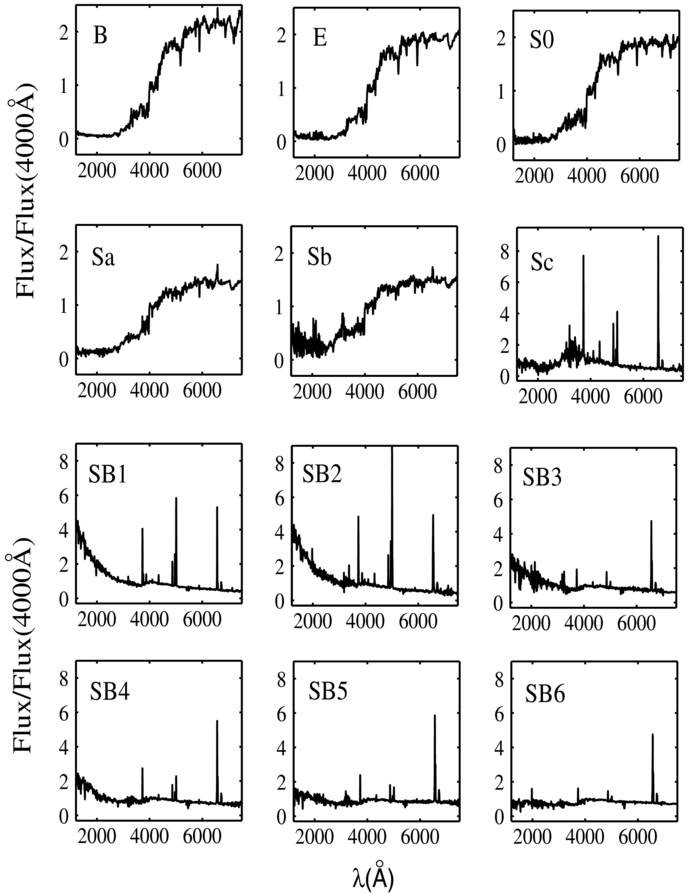
\includegraphics[width=0.47\textwidth]{images/k96.jpg}
        \caption {\citet{Kinney96} spectral templates for 12 types of galaxies, from fig. 1 in \citet{Hossein12}. The type of each template is shown in each frame. Plots B, E, S0, Sa, Sb and Sc show spectra that belong to quiescent galaxies. Starburst galaxy spectra are indicated with SB1 to SB6. Higher numbers represent more intrinsic extinction. Note that the vertical axis label from \citet{Hossein12} is incorrect:  the quantity plotted in the vertical axis is flux density, not flux.}
        \label{fig: k96}
    \end{figure}
      
    \citetalias{Kinney96} used ultraviolet-optical spectra of 70 star-forming and quiescent nearby galaxies to produce a set of templates that contained 12 types of spectral templates.
    These templates have been widely used in many studies to determine morphological type of galaxies or properties of specific types of galaxies~\citep[e.g.][]{Shakouri16, Paiano16, Laporte16, Holden16}.
    \citetalias{Kinney96} stated that these templates can also be used to classify the spectra of high-redshift galaxies. 
    
    The 12 templates are divided based on their morphological types for quiescent galaxies or their extinction for starburst galaxies (Fig.~\ref{fig: k96}). 
    The quiescent group of galaxies includes Bulge (B), Elliptical (E), S0, Sa, Sb, and Sc galaxies.
    The bulge group represents galaxies similar to M31 and M81, whose UV and optical spectra are dominated by their bulge stellar populations.
    The starburst galaxies are divided into six groups (SB1 to SB6) based on their intrinsic extinctions ($E(B-V)$). 
    As Fig.~\ref{fig: k96} shows, SB1 galaxies have lower internal extinctions ($E(B-V) \simeq 0.05$), while SB6 galaxies have the highest amount of extinction ($E(B-V) \simeq 0.65$) among starburst galaxies. 
    In the quiescent (B to Sb) templates, the spectrum is redder; strong absorption lines and the 4000~\AA~break are distinguishable.
    The SEDs of starburst galaxies are flatter in the optical and near-infrared region than those of the quiescent ones and show strong emission lines.
    For more details on each spectral type, we encourage readers to see \citetalias{Kinney96} and references therein. 
   The \citetalias{Kinney96} spectra span from $\sim1200$~\AA~to $10000$~\AA~with a resolution of $\sim 10$~\AA.
    However, in this work we only use observations in the rest-frame wavelength range $\sim1200< \lambda < 8000$~\AA~to train our networks; 
    this wavelength range was chosen due to the availability of flux information in those wavelengths for all 12 templates. 

 \subsection{SED and Properties of the Sample Galaxies} 
    \citetalias{Hossein12} selected 142 galaxies from the spectroscopic campaign of the ESO GOODS-South field~\citep{Vanzella05, Vanzella06, Vanzella08}.
    The 142 galaxies were selected based on the availability of photometry from HST/ACS, VLA/ISAAC, and {\it Spitzer}/MIPS and IRAC (10--13 filters with $\sim 0.4<\lambda<24~\mu$m in the observed frame).
   Data from these instruments was necessary in order to have a complete picture of stellar population and star formation rate. 
    For each galaxy, a robust spectroscopic redshift and photometric measurements from the GOODS-MUSIC catalogue \citep{Santini09} were available.
\citetalias{Hossein12} used point-spread-function matched photometry 
    from \citet{Santini09} as input to the Code Investigating GALaxy Emission ({\em CIGALE});~\citep[][hereafter N09]{Noll09} to generate the best-fit SED for each galaxy.
    \citetalias{Hossein12} produced the best SED match, with the wavelength interval of 910~\AA~to $\sim 80$~cm, for each galaxy\footnote{This wavelength interval is the default output of the {\em CIGALE} code.}.
    Assuming decreasing SFR and visual attenuation ($\tau$) model, Salpeter initial mass function~\citep{Salpeter55}, and an old stellar population with age of $\sim 10$~Gyr, he derived physical properties of the galaxies such as age and stellar mass.
    Some of these properties are shown in Table~\ref{tab: props}.
    In Section~\ref{sec: 1D_somz}, we study these properties for each category.
    More details on creating SEDs and extracting information about galaxy properties using {\em CIGALE} can be found in \citetalias{Noll09} and \citetalias{Hossein12}.
    
       
\begin{table}
\caption[Description of the properties of \citet{Hossein12} galaxies]{Description of the properties of \citet{Hossein12} galaxies; the output result of {\em CIGALE}}     
\label{tab: props}
\centering
\begin{tabular}{l l l}
\hline\hline
\noalign{\smallskip}
Par. & Unit & Description\\
\noalign{\smallskip}
\hline
\noalign{\smallskip}
$f_\mathrm{burst}$ & --- & mass fraction of \\
& & young single population (SP) model \\
\noalign{\smallskip}
$t_{\,\mathrm{oSP}}$ & Gyr & age of old SP model \\
$t_{\,\mathrm{ySP}}$ & Gyr & age of young SP model \\
$t_{\,\mathrm{D4000}}$ & Gyr & D4000-related age \\
\noalign{\smallskip}
$M_\mathrm{star}$ & M$_\odot$ & total stellar mass  \\
SFR & M$_\odot$/yr & instantaneous SFR  \\
$A_\mathrm{FUV}$ & mag & attenuation at 1500\,\AA{} \\
\noalign{\smallskip}
\hline
\end{tabular}
\end{table}

    We classify SEDs that were produced by \citetalias{Hossein12} using the created networks.
    These SEDs are publicly available\footnote{All the SEDs produced by \citetalias{Hossein12}  can be found at this \href{http://telbib.eso.org/detail.php?bibcode=2012AJ....144..172T}{ESO webpage}.} in the form of flux per rest frame wavelength over a wide range of wavelengths.
    Since we have chosen the \citetalias{Hossein12} SEDs to be classified by the trained network, we only used the part of the SEDs that have the same wavelength range as the \citetalias{Kinney96} spectral templates.  